\chapter{Quantum Programming Languages}
\label{QPL}

\epigraph{\textit{A new breed of quantum programmer is needed to study and implement quantum software — with a skillset between that of a quantum information theorist and a software engineer.}}{Will Zeng\\ Rigetti Computing \cite{WZ2017}}

%%%%%%%%%%%%%%%%%%%%%%%%%%%%%%%%%%
%%%%%%%%%%%%%%%%%%%%%%%%%%%%%%%%%%

I think here we should thoroughly explain the syntax of each language with a basic example implementation.  with examples (not Deutsch cause we haven't explained it yet). I propose I super simple example, like generating a superposition state and performing some measurements.

For each language need to talk about the following:
\begin{itemize}
\item How is the program structured? (E.g. as a quantum processor/subprogram to regular programming language)
\item Qubit, Ancilla bits, Classical bits
\item How are gates applied?
\item How are measurements handled?
\item Available libraries
\item Available for which operating systems
\item Use case of language and future of language
\item Support available
\item Flexibility of language (hardware, simulation, cost estimator, etc.)
\end{itemize} 

%%%%%%%%%%%%%%%%
%%%%%%%%%%%%%%%%
%%%%%%%%%%%%%%%%
%%%%%%%%%%%%%%%%
\section{Rigetti - pyQuil}
%%%%%%%%%%%%%%%%
%%%%%%%%%%%%%%%%
%%%%%%%%%%%%%%%%
%%%%%%%%%%%%%%%%

In this section we address the main features of the programming language by Rigetti and the description of its syntax with a simple example.

pyQuil is the Python based programming language created by Rigetti \cite{pyQuilDoc} as part of their quantum programming toolkit for their hardware. This consists of
\begin{itemize}
    \item \textbf{Forest} - Rigetti's entire quantum programming toolkit. 
    \item \textbf{Quil} – Quantum Instruction Language which is assembly-like as it lists the gates to apply. Acts as an intermediate step between pyQuil and the actual instructions that will go to the quantum computer.
    \item \textbf{pyQuil} - Open source Python library. The user writes their code in pyQuil and this gets translated to Quil.
    \item \textbf{QVM} - Rigetti's Quantum Virtual Machine which runs simulations of up to 26 qubits, an API key is required to access this.
    \item \textbf{QPU} – Quantum Processing Unit, Rigetti's actual chip with 19 qubits which requires special access.
    \item \textbf{Grove} - Open source Python library containing quantum algorithms developed with pyQuil. 
\end{itemize}

\begin{figure}[H]
    \centering
    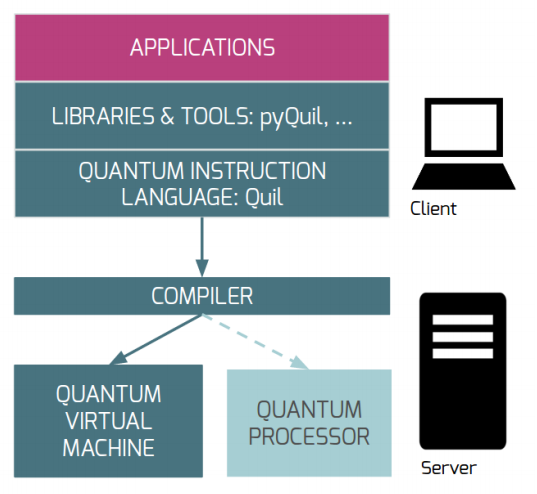
\includegraphics[width=0.5\textwidth]{Forest_structure.PNG}
    \caption{The structure of Forest. Figure taken from \cite{Rigetti2016} - possibly need to create our own}
    \label{fig:my_label}
\end{figure}

A program would be written in pyQuil which gets translated to Quil. If the program is being run on the QVM, it is generally not necessary to decompose the Quil instructions further since the code is being run on a simulator and everything comes down to mathematical operations. If the program is to be run on the QPU, a compiler will break down the Quil instructions into quantum gates which can be executed on the actual chip. This is necessary because QPUs currently have a more limited gate set due to the technology used to create the chip. For example if you would like to perform a controlled-NOT gate, this may have to be broken down into the elementary gates for the specific chip architecture.  

Quil has been designed with the idea in mind that near term quantum computers will act as co-processors along with classical processors. It can execute quantum programs with classical control. pyQuil is more of a high-level language, hence in the guide we will be focusing on this rather than Quil.   

%%%%%%%%%%%%%%%
%%%%%%%%%%%%%%%
\begin{comment}

The Rigetti-Forest toolkit \cite{Rigetti2016} for hybrid classical-quantum computing uses the language called Quil. The python library called pyQuil allows us to run simulations in their Quantum Virtual Machine (QVM) which allows the simulation up to 26 qubits, and to run simulations on their Quantum Processor Unit (QPU) which is the physical device called 19Q Acorn which have 20 physical qubits, of which 18 are logical. They recently made available a ~100 pages pyQuil documentation \cite{pyQuilDoc} with examples and exercises to be implemented whether in the QVM or QPU. Access to the QVM can be granted to everyone by registering in their website (they send you an API key right away).

\end{comment}

%%%%%%%%%%%%%
%%%%%%%%%%%%%
%%%%%%%%%%%%%%%%%%%%%%%%%%%%%%%%%%%%%%%%%
%%%%%%%%%%%%%%%%%%%%%%%%%%%%%%%%%%%%%%%%%
%%%%%%%%%%%%%%%%%%%%%%%%%%%%%%%%%%%%%%%%%
\subsection*{Quantum Programs with pyQuil} 
\label{Quantum Programs with pyQuil}
%%%%%%%%%%%%%%%%%%%%%%%%%%%%%%%%%%%%%%%%%
%%%%%%%%%%%%%%%%%%%%%%%%%%%%%%%%%%%%%%%%%
%%%%%%%%%%%%%%%%%%%%%%%%%%%%%%%%%%%%%%%%%

Quantum algorithms require the implementation the three computational stages. We first need to initialise the state in a state of the form $\ket{00...0}$, we then need to apply gates in order to obtain a target state of interest and finally, we perform measurements in the computational basis. Let us see how to address these stages with the following specific example.

%%%%%%%%%%%% title= Example 1
\begin{tcolorbox}[standard jigsaw,
    opacityback=0,  % this works only in combination with the key "standard jigsaw"
    boxrule=0.5pt,label={example1}]
    {\bf Example 1}
    \tcbline
    Generating the one-qubit pure state 
    \begin{align*}
    \ket{\psi\left(\phi\right)}=\frac{1}{\sqrt{2}}\left(\ket{0}+e^{i\phi}\ket{1}\right),
    \end{align*}
    by applying gates to the initial state $\ket{0}$ and performing measurements.
\end{tcolorbox}
%%%%%%%%%%%%%%%
Starting with the one-qubit state $\ket{0}$, we can generate the superposition with a Hadamard gate, and we then can add the desired phase with a gate of the form $here$. Finally, we consider projective measurements. We remark here however, that these steps can be implemented in any programming language that handles linear algebra.  We can do it in python with the Python library Numpy in the following way \autoref{lst:ExamplePython}.

%\columnbreak
%%%%%%%%%%%%%%%%%
\begin{lstlisting}[language=Python,caption={Example with python only},label={lst:ExamplePython},frame=single] 
import numpy as np
# State initialisation
state0=np.array([[1],[0]])
# State manipulation
H=(1/np.sqrt(2))*np.array([[1,1],[1,-1]])
state1=np.dot(H,state0)
phi=np.pi/2
PHASE=np.array([[1,0],[0,np.exp(1j*phi)]])
state2=np.dot(PHASE,state1)
# Measurement: defining projectors P0,P1
ket0=np.array([[1],[0]])
ket1=np.array([[0],[1]])
P0=np.dot(ket0,ket0.T)
P1=np.dot(ket1,ket1.T)
# Probability of obtaining outcome 0
prob0=np.trace(np.dot(P0,np.dot(state2,np.conj(state2).T)))
# Probability of obtaining outcome 1
prob1=np.trace(np.dot(P1,np.dot(state2,np.conj(state2).T)))
\end{lstlisting}
%%%%%%%%%%%%%%%%
However, this is local, and we are running this computation in our standard computers and therefore is a classical simulation of a quantum computation.

We would like to implement this in a real quantum computer, and this is where Rigetti comes in. We need further software to manipulate real QPUs, and therefore cannot be as straightforward as our previous code. but we are using the QVM.

%\columnbreak

{\bf 0. Libraries:} The connection and qubit initialisation of our qubits is given by:
\begin{lstlisting}[language=Python]
from pyquil.quil  import Program 
from pyquil.api   import QVMConnection 
from pyquil.gates import I,X,Z,Y,H,PHASE
import numpy as np
\end{lstlisting}

{\bf 1. Initialisation:} The systems has been initialised into a state of $n$
 qubits in the $|00...0>$ state. Of course both the qvm and qpu are limited by this and that respectively.\\ 
 
 the other point is that this is a lst of instructions and the actual computation has not taken place, and we need to invoke the command run to do it.\\
\begin{lstlisting}[language=Python,firstnumber=5] 
# Invoking and renaming
qvm=QVMConnection()
p=Program()
\end{lstlisting} % numbers=none 
 
 %%%%%%%%%%%%%%%%%%%%%%%%%%%%%
 {\bf 2. Gate implementation:} So far we have only covered initialisation, now we need to consider state manipulation. The way that gates are being called is as follows:
 %%%%%%%%%%%%%%%%%
\begin{lstlisting}[language=Python,firstnumber=8]
# Gate implementation
p.inst(H(0))
theta=np.pi/2
\end{lstlisting}
%%%%%%%%%%%%%%%%
 by considering the object program which we have renamed as p with the methd isnt we apply fro left to right in order of application and inside parenthesis the qubit which is acting upon the qubits are listed from $0,1,...n$. For instance applying gates this and that. The complete set of gates can be found in HERE.\\
 
%%%%%%%%%%%%%%%%%%%%%
{\bf 3. Measurement:} Yadda describing 
\begin{lstlisting}[language=Python]
# Measurement
p.measure(0,0)
p.measure(1,1)
\end{lstlisting}
 
%%%%%%%%%%%%
{\bf 4. Run:} So far this is only a list, now finally we run the program with the command.
\begin{lstlisting}[language=Python]
# Running the program
cr=[]
results=qvm.run(p,cr,4)
print(results)
\end{lstlisting}
So in full our program looks like this \autoref{lst:ExampleQVM}.
%%%%%%%%%%%%%%%%%
\begin{lstlisting}[language=Python,caption={Example algorithm implemented with pyQuil.},label={lst:ExampleQVM},frame=single] 
from pyquil.quil  import Program 
from pyquil.api   import QVMConnection 
from pyquil.gates import H,PHASE
import numpy as np
# Invoking and renaming
qvm=QVMConnection()
p=Program()
# Gate implementation
p.inst(H(0))
theta=np.pi/2
p.inst(PHASE(theta,0))
# Measurement
p.measure(0,0)
p.measure(1,1)
# Running the program
cr=[]
results=qvm.run(p,cr,4)
print(results)
\end{lstlisting}

%In this section we address the main features of the programming language by (QISKit company) and the description of its syntax with a simple example.

%%%%%%%%%%%%%%%%%%%%%%%%%%%%
\section{IBM - QISKit}
%%%%%%%%%%%%%%%%%%%%%%%%%%%%

IBM has launched the IBM Q experience that consists of a development environment called QISKit, a higher-level gate-building software development kit (SDK) that allows users to compose their own quantum algorithms, and OpenQASM, a low level quantum assembly language to realise the gates at the quantum prosessing unit (QPU). The devices used to perform the simulation and computation are based on a superconducting charge qubit implementation, which can be found described in more detail in \autoref{Implementations}. \\
\indent There is ample space for development of algorithms in this environment as the visual arrays provide a clear structure to those familiar with quantum computation. The composer also displays the code on which it operates so that users interested in further development have the opportunity to learn how to code their own gates in OpenQASM as well as QISKit. The associated documentation which is linked on the IBM Q website provides more detail to the structure \cite{coles2018quantum}. \\
\indent The architectures (physical or virtual) that the user can execute their quantum algorithms on are easily accessible via the IBM Q Experience web page, and can be seen in \autoref{fig:ibmsite}. IBM recently published a report detailing their state-of-the-art prototype 50 qubit chip in the 2017 IEEE ICRC conference \cite{ibm50}.\\

The current state of IBM's stack, from top to bottom consists of the following elements:

\begin{itemize}
    \item \textbf{QISKit} - IBM's open source quantum library for usage in the high level language Python. 
    \item \textbf{QISKit ACQUA} - IBM's open source, modular Algorithms and Circuits for Quantum Applications library for usage in the high level language Python. The modules in this library as specifically targeted towards industry professionals in the research areas of Chemistry, artificial intelligence and optomization. 
    \item \textbf{OpenQASM} – IBM's low-level Quantum Assembly Language which interprets commands and functions from QISKit and translates them into microwave pulses for use on the physical architecture (superconducting qubits). Acts as an intermediate step between QISKit and the actual instructions that will go to the quantum computer.
    \item \textbf{QPU} - IBM has multiple physical architectures for running quantum algorithms. These include 3, 4, 5 and 16 qubit devices accessible via an API provided when you create an account with the IBM Experience, and larger 20 qubit devices that are available via membership to the IMB Q Network (hubs, partner institutions etc).
    \item \textbf{Q QASM Simulator} - IBM's Quantum Virtual Machine which runs simulations of up to 32 qubits, an API key is required to access this.
\end{itemize}
%%%%%%%%%%%%%%%%%%
\begin{figure}[h!]
\centering
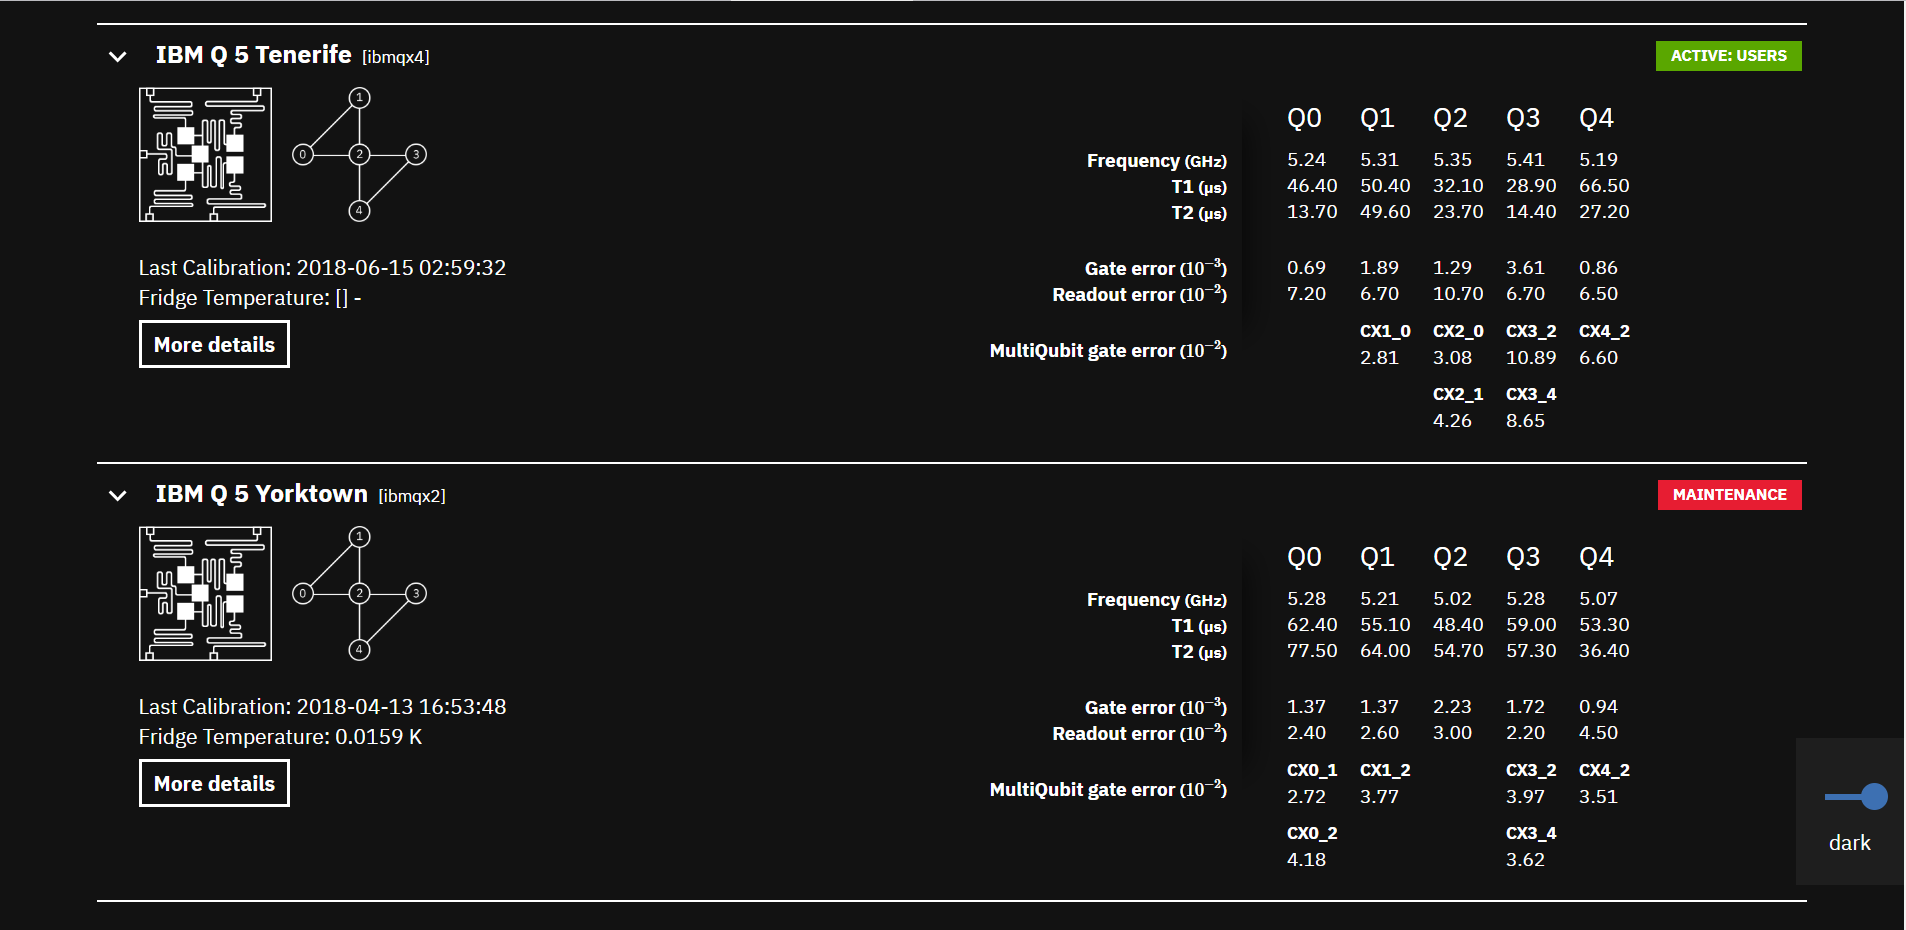
\includegraphics[width=\textwidth]{IBMq_1}
\caption{The description of the devices used for the IBM Q suite (to be updated closer to submission). Cooling refrigerator temperature along with the update structure is presented. A useful live display feed allows users to track both the physical and computational side of their own algorithms made on the composer.}
\label{fig:ibmsite}
\end{figure}

%%%%%%%%%%%%%%%%%%%%%%%%%%%%%%%%%%%%%%%%%
%\subsection{QISKit General Description}
%%%%%%%%%%%%%%%%%%%%%%%%%%%%%%%%%%%%%%%%%

%%%%%%%%%%%%%%%%%%%%%%%%%%%%%%%%%%%%%%%%%
\subsection*{Quantum Programs with QISKit}
%%%%%%%%%%%%%%%%%%%%%%%%%%%%%%%%%%%%%%%%%

The first basic example of QISKit will be to generate a single qubit superposition, $\ket{\psi}=\frac{1}{\sqrt{2}} \left(\ket{0}+e^{i\phi}\ket{1}\right)$, beginning with the all qubits in the state $\ket{0}$. We will focus on the cases of $\phi=0$ and $\phi = \pi$. These can be broken down into the action of the Hadamard operator on $\ket{0}$ and the Hadamard operator followed by the Z Pauli gate. These actions are written in \autoref{eq:H1} and \autoref{eq:ZH}, respectively.

\begin{equation}
    H\ket{0}=\frac{1}{\sqrt{2}}\left(\ket{0}+\ket{1}\right)
    \label{eq:H1}
\end{equation}
\begin{equation}
    ZH\ket{0}=\frac{1}{\sqrt{2}}\left(\ket{0}-\ket{1}\right)

    \label{eq:ZH}
\end{equation} 
We can simulate both of these actions on the composer in the IBM Q experience, or use experiment tokens to run the program on the processor IBM provides (referred to as ibmqx4) as seen in \autoref{fig:ZH}. 

\begin{figure}[h!]
    \centering
    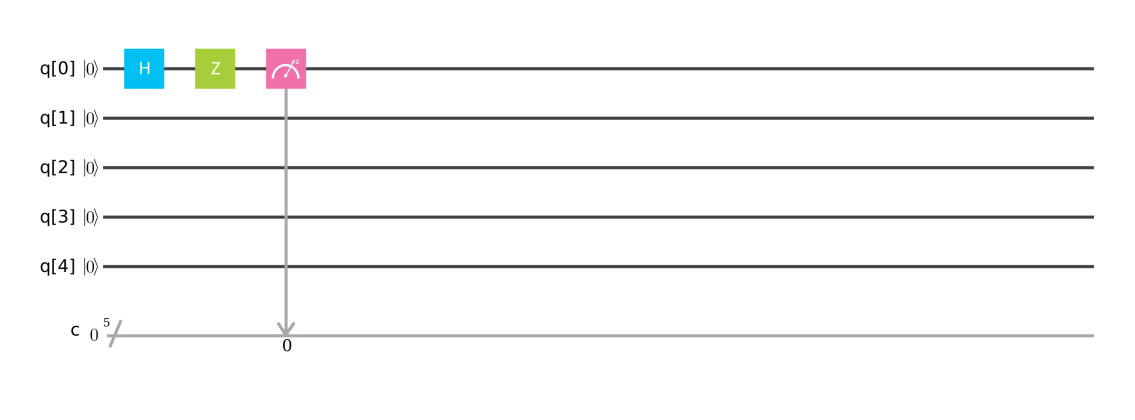
\includegraphics[width=\textwidth]{ZHcodecomposer}
    \caption{The composer view of the code that we can use to simulate the generation of $ZH\ket{0}=\frac{1}{\sqrt{2}}\left(\ket{0}-\ket{1}\right)$.}
    \label{fig:ZH}
\end{figure}

Though the composer is a useful place to get started with your own simulations of basic gate operations, it doesn't give us a an opportunity to truly experiment with the hardware at a deeper level. To do this, we need to start experimenting with the QISKit language itself.

\begin{figure}
    \centering
    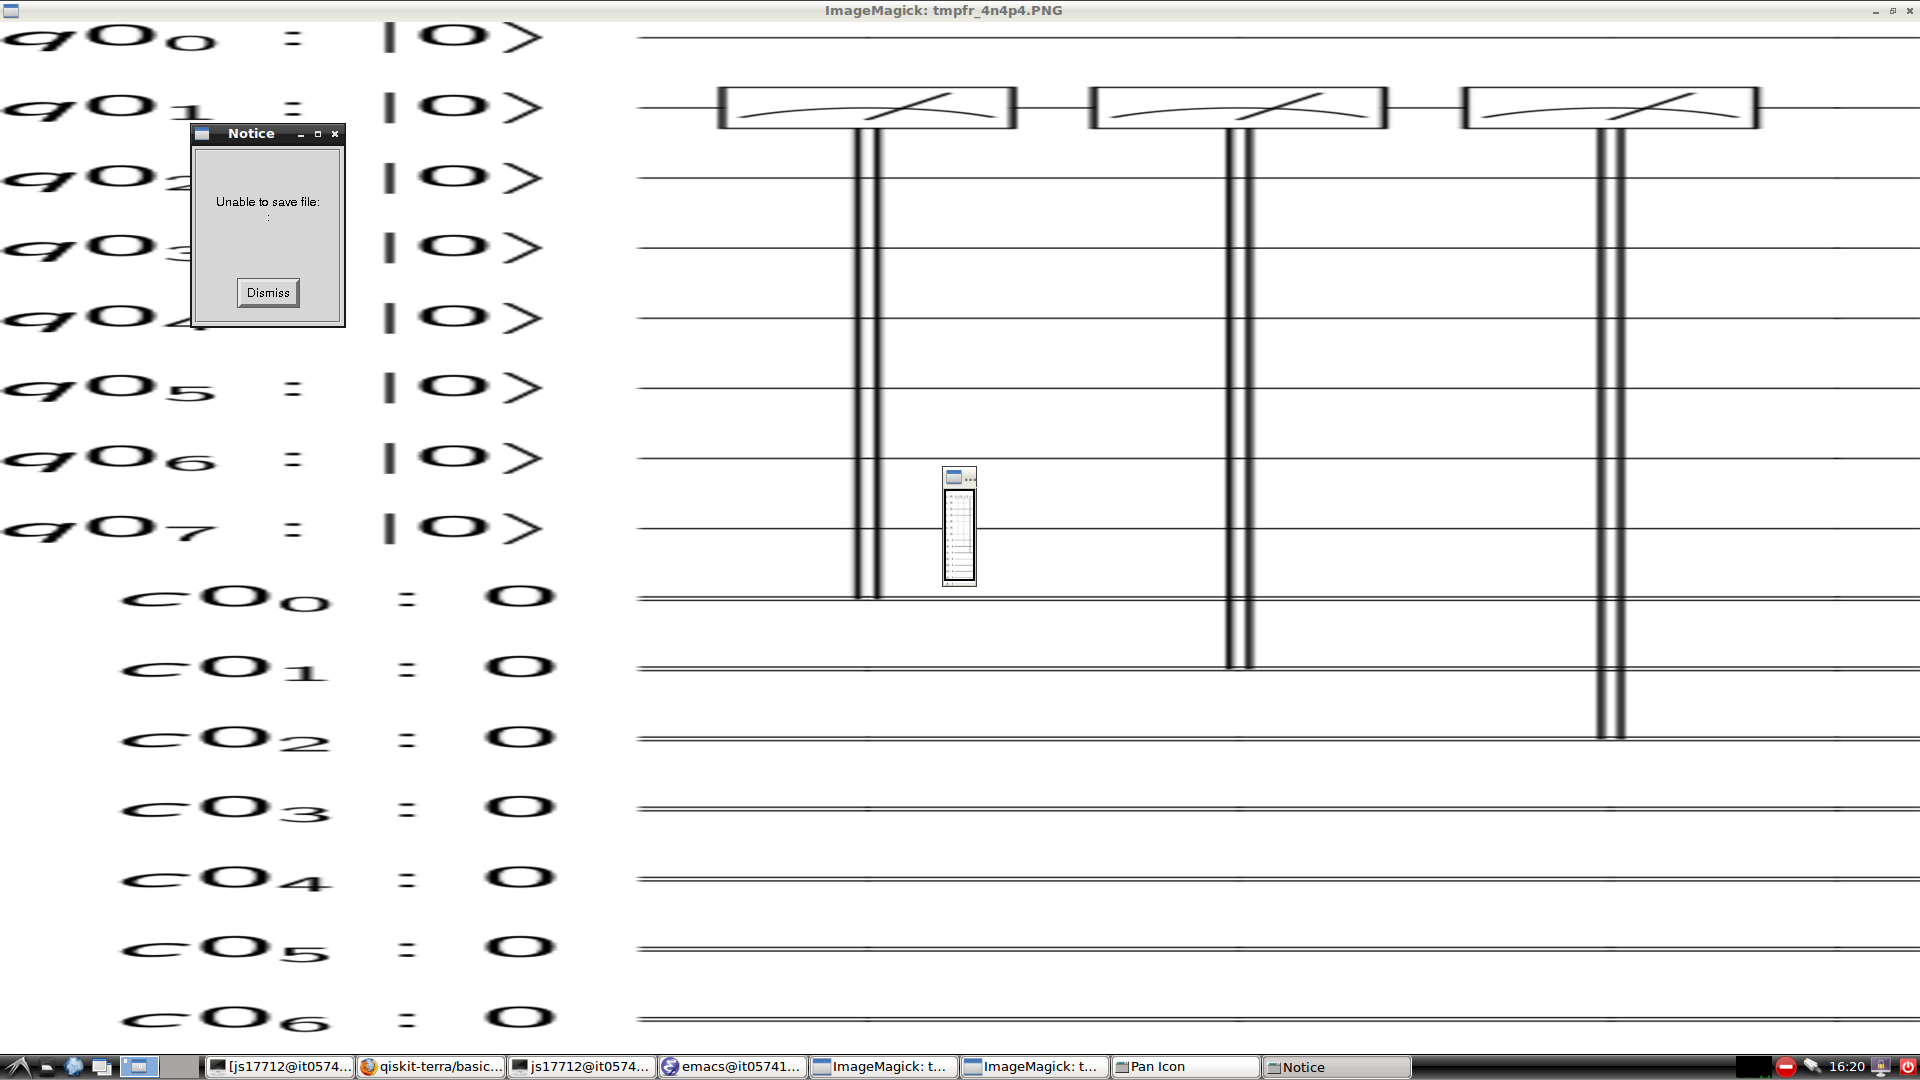
\includegraphics{the_qanswer.png}
    \caption{Caption}
    \label{fig:my_label}
\end{figure}

Consider the previous example illustrated by the gate composer in \ref{fig:ZH}. This relatively simple example can be expanded upon in QISKit via the generation and measurement of a Bell state, described by \autoref{eq:BS}

\begin{equation}
    \ket{\psi}=\frac{1}{\sqrt{2}}\left(\ket{01}+\ket{10}\right)
    \label{eq:BS}
\end{equation} 

To create this state, and measure it on IBM's Q QASM Simulator, the follwoing code can be utilised:
\newpage

\begin{lstlisting}[language=Python,caption={Example algorithm implemented with QISKit.},label={lst:ExampleQQASM},frame=single] 
# Program written using QISKit to demonstrate the way in which to create an equal weighted
# superposition of states in the computational basis, and then simulate the measurement
# on IBM's Q QASM simulator

# Import relevant library functions from QISKit
from qiskit import ClassicalRegister, QuantumRegister, QuantumCircuit
from qiskit import available_backends, execute

# Initiate quantum registers for gate execution, and classical registers for measurements
q = QuantumRegister(2)
c = ClassicalRegister(2)
qc = QuantumCircuit(q, c)

# Preform a Hadamard on the qubit in the quantum register to create a superposition
qc.h(q[0])
# Preform a controlled-not operation between the first and second qubits in the register
qc.cx(q[0], q[1])
# Preform an X-pauli on the second qubit in the register
qc.x(q[1])
# Measure the superposition
qc.measure(q, c)

# Check simulation backends
print("Local backends: ", available_backends({'local': True}))

# Submit the job to the Q QASM Simulator (Up to 32 Qubits)
job_sim = execute(qc, "local_qasm_simulator")
# Fetch result
sim_result = job_sim.result()

#Print out the simulation measuement basis and corresponding counts
print("simulation: ", sim_result)
print(sim_result.get_counts(qc))
\end{lstlisting}

When ran, the output produced is as follows:

\begin{lstlisting}[language=Python,caption={Bell State generation and measurement output.},label={lst:ExampleQQASMoutput},frame=single] 
Local backends:  ['local_qasm_simulator', 'local_statevector_simulator', 'local_unitary_simulator']
simulation:  COMPLETED
{'01': 513, '10': 511}
\end{lstlisting}

Here, the back end in selected in line 1, completion confirmation is shown in line 2, and the measurement basis and counts are shown in line 3, illustrating that indeed the Bell State specified in \ref{eq:BS} has been generated, and measured. 
\newpage


%%%%%%%%%%%%%%%%%%%
%%%%%%%%%%%%%%%%%%%
\section{ProjectQ}

ProjectQ is an open source Python based language. ProjectQ can run on a local simulator - your computer. But there is also an option to connect to the IBM back-end to run code on their simulator or chips, and this may be extended to other hardware in the future as well. This makes ProjectQ a general quantum programming language that is not platform specific unlike pyQuil, QISKit and Q\#.  

\begin{figure}[H]
    \centering
    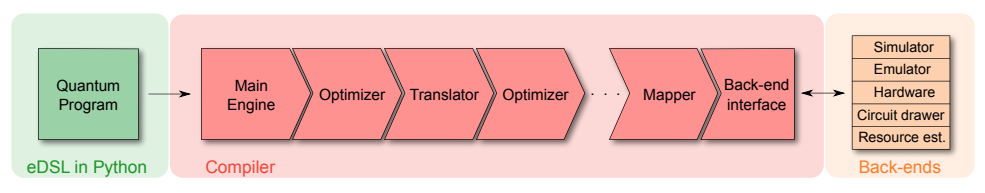
\includegraphics[width=\textwidth]{projectq_structure.PNG}
    \caption{Structure of ProjectQ. Taken from \cite{projectq2018}, will make own diagram and possibly simplify.}
\end{figure}

ProjectQ is one of the more flexible quantum programming languages available in terms of the types of operations, compilers and back-ends that are available. Many of the typical gates that are used in quantum algorithms are already built in, and user defined gates that are either just matrices or based on mathematical operations are relatively simple to implement. 

The compiler is designed to have a modular structure, so the user can pick and choose the level of optimisation required. 

% Note: This section is not finished! I will complete the compiler paragraph and discuss the different back-ends etc. 

%%%%%%%%%%%%%%%%%%%%%%%%%%%%%%%%%%%%%%%%%%%
\subsection*{Quantum Programs with ProjectQ}
%%%%%%%%%%%%%%%%%%%%%%%%%%%%%%%%%%%%%%%%%%%

% I may add another example to this section since it is quite short. Or do things need explaining in more detail?

We will now do a simple demonstration in ProjectQ to create the superposition $\frac{\ket{0}+\ket{1}}{\sqrt{2}}$. 

\lstinputlisting[language=Python]{code/ProjectQ/superpos_projectq.py}

The first thing to do is to set up the back-end that the program will be run on. This is done by calling \texttt{MainEngine} which has the local simulator as the default back-end, this can also be set up to be the IBM back-end or something else such as a resource estimator.

Qubits can now be allocated, either individually (as shown above) or as a register, from the \texttt{engine}. The syntax to do an operation is  \texttt{Gate | Qubits}. Finally the gates are sent to the compiler by use of the \texttt{flush} command. And if you wish to display the result, the qubit can be converted to type integer after measurement.


\newpage
%%%%%%%%%%%%%%
%%%%%%%%%%%%%%
\section{Q\#}
%%%%%%%%%%%%%%
%%%%%%%%%%%%%%
One of the languages that is strongly quantum platform independent is Q\#. It is being developed by Microsoft and very roughly based on their classical languages C\# and F\#. It is, however, not just a library, but designed to be its own language. Q\# is developed to be a high-level quantum programming language. Though it still allows the basic single qubit operations, it also provides a more advanced library and allows user-defined ``operations" which can be used to structure more complicated programs. The programming language should be platform independent to allow users to write programs now for quantum computers available in the future. Currently it runs on a simulator (either on your local computer or Azure, a Microsoft cloud computing service) or a cost estimator (trace simulator) which approximates qubit and gate requirements for the program. \\
The concept behind the language is that the quantum computer is treated like a coprocessor: like GPU is a graphical coprocessor, a QPU is the quantum one. This means that a program using the QPU requires a driver program, which controls the main processor (CPU) and which then calls on a subprogram controlling the QPU. The QPU program in this case will be written in Q\#, whereas the driver program can be written in not just C\# or F\#, but any language supporting the .NET framework. In this programming guide the driver programs are written in C\#, but you could easily change this if you are more comfortable with another language.\\
As Q\# is dependent on the .NET framework, it is currently only available for Windows computers. The easiest way to get started is probably by programming with Visual Studio. Tutorials for installing this API and Q\# can be found online. \\
Q\# comes with a standard library which is divided into two sections: The basic building blocks of the language, such as the qubit and measurements representations and the operations given above, are part of the so-called prelude. The prelude is dependent on the target machine, e.g. a simulator.  The second part, called the canon, is machine independent and built on the elements that form the prelude. It gives implementations of various quantum algorithms such as a quantum Fourier transform and a phase estimation.  

\paragraph{Basic building blocks} There are several primitive types specific to Q\# and an overview of these is given in table \ref{table:PrimTypeQsharp}. The first five are analogous to types in classical programming languages, e.g. C\#. The others are more quantum programming specific. \\
It is also possible to create arrays, e.g. a \texttt{Qubit[]} or an \texttt{Int[][]}. Tuples, so e.g. (a, b, c), are also used. a, b and c could be of different types and tuples can be quite useful in returning multiple values from an operation. You can also define your own types, but they must be based on the primitive types.\\
Another thing a Q\# programmer has to keep in mind, is that variables are normally immutable. Values are assigned with a \texttt{let} statement and they cannot be changed afterwards. To allow changing the value of a variable one can use the \texttt{mutable} keyword when assigning a value to a variable. Changing the variable is then done with the \texttt{set} statement.\\
Qubits are maybe the most important resource in a quantum program. You cannot assign a value to a \texttt{Qubit}, but you can measure it and then apply operations to change it to the value you want. The default value of a \texttt{Qubit} is $\ket{0}$, i.e. the computational \texttt{Zero} state, and it is generally good practice to reset a used \texttt{Qubit} to this before releasing it.\\
The easiest way to use actually use \texttt{Qubit}s is to write a \texttt{using} statement, e.g. \texttt{using (qubits = Qubit[2])\{<any code using these qubits>\}}.

\begin{table}[!htb]
      \centering
        \begin{tabular}{|l|l|}
        \hline
        Type    & Values \\ 
        \hline
        \texttt{Int}     & 64-bit signed integer \\
        \texttt{Double}  & double-precision floating-point number \\
        \texttt{Bool}    & Boolean value (\texttt{true} or \texttt{false}) \\
        \texttt{String}  & Unicode sequence, used to pass messages to classical driver program\\
        \texttt{Range}   & sequence of integers\\
        \texttt{Qubit}   & qubit\\
        \texttt{Result}  & outcome of measurement (\texttt{One} or \texttt{Zero})\\
        \texttt{Pauli}   & elements of the Pauli group (\texttt{PauliI}, \texttt{PauliX}, \texttt{PauliY} or \texttt{PauliZ})\\
        \hline
    \end{tabular}
    \caption{Primitive types in Q\#}
    \label{table:PrimTypeQsharp}
\end{table}

%%%%%%%%%%%%%%%%%%%%%%%%%%%%%%%%%%%%%%%%%
\subsection*{Quantum Programs with Q\#}
%%%%%%%%%%%%%%%%%%%%%%%%%%%%%%%%%%%%%%%%%
Q\# programs require two main bits of code: a ``classical" driver program and the quantum program. The driver program here is in C\#, but as mentioned in the previous section this could be another language. It must use two namespaces: \texttt{Microsoft.Quantum.Simulation.Core} and \\ \texttt{Microsoft.Quantum.Simulation.Simulators}. Next you want to define the namespace you want to work in: in this case Quantum.Superposition, which will be shared by your driver and your quantum program.\\
Then you start your driver program like you would any regular program. In C\# you create a class and the entry point for the program is your \texttt{static void Main(string[] args)} method.\\
As we do not have an actual QPU, we are using a simulator. To create an instance of the simulator in your program you can use a \texttt{using} block. This creates the simulator instance and ensures it is disposed of when the block ends.\\
In the "using" block you can then call on the quantum operation defined in your quantum subprograms. In this case that will be the operation "Superposition". The operation is actually run with the method \texttt{Run(<QuantumSimulator>, arg1, arg2, ...)}, where the \texttt{arg} arguments are any potential arguments passed to the quantum operation. In this simple example the quantum operation does not take any arguments so we are only passing the Quantumsimulator \texttt{sim} to \texttt{Run}. Finally, we want to actually get the outcome of the quantum operation, which we get by adding \texttt{.Result} to the end.\\
Then the rest of the driver program can be completely classical again, with the exception that the objects returned can be specific quantum types.\\


\begin{lstlisting}[language=Csharp,caption={Starting a driver program for Q\#},label={lst:C\#driverSimple}] 
using Microsoft.Quantum.Simulation.Core;
using Microsoft.Quantum.Simulation.Simulators;

namespace Quantum.Superposition{

    class Driver{
        static void Main(string[] args){

            using (var sim = new QuantumSimulator()) {
                Result outcome = Superposition.Run(sim).Result;
                System.Console.WriteLine
                        ($"Measuring equal superposition state gave outcome {outcome}.");
            }

            System.Console.WriteLine("Press any key to continue...");
            System.Console.ReadKey();
        }
    }
}
\end{lstlisting}

To specify the quantum operation you need to write Q\# code. Again, you start by defining the namespace we are working in (\texttt{Quantum.Superposition}). Next there are two namespaces you will need to use, which are specified with the keyword \texttt{open} (similar to \texttt{using} in C\#): \\ \texttt{Microsoft.Quantum.Primitive} and \texttt{Microsoft.Quantum.Canon}.\\
New operations are defined with the keyword \texttt{operation} and the arguments taken and the return value is specified here in the form \texttt{operation OperationName (arg1: type1, arg2: type2, ...) : (returnType)}.
Inside the operation you define the actual steps to take in the \texttt{body} block. \\
Here we are defining a mutable variable res. It is assigned the value \texttt{Zero}, which is of type \texttt{Result}. This variable will be used to return the outcome of the quantum operation. Next, a \texttt{Qubit} array containing one \texttt{Qubit} is created and after applying a Hadamard (\texttt{H}) gate the \texttt{Qubit} will be in state $\frac{\ket{0}+\ket{1}}{2}$. Then the \texttt{Qubit} is measured (\texttt{M}) and afterwards returned to the $\ket{0}$ state. The measurement outcome is then returned to the driver program. \\
One thing to note here is that we needed to define the variable \texttt{res} outside the \texttt{using} block, as any variables defined in the block are local only to the \texttt{using} block. We cannot use the return statement inside the \texttt{using} block either, so we needed to use a variable local to the whole \texttt{body} block to return a value from the operation.\\

\begin{lstlisting}[language=Qsharp,caption={A simple program in Q\# creating and measuring an equal superposition.},label={lst:Q\#Simple}]
namespace Quantum.Superposition{

    open Microsoft.Quantum.Primitive;
    open Microsoft.Quantum.Canon;

    operation Superposition() : (Result){

      body{

        mutable res = Zero;

	    // create a qubit reqister
	    using (reg = Qubit[1]){
	      // Apply the Hadamard gate to your qubit to create an equal superposition
          H(reg[0]);

	      // Measure the qubit in superposition
	      set res = M(reg[0]);

	      // Reset the qubit to its clean |0> state
	      if (res == One){
	        X(reg[0]);
	      }
	    }

      return res;
            
      }
    }
}
\end{lstlisting}

%%%%%%%%%%%%%%%%%%%%%%%%%%%
\section{Further languages}
%%%%%%%%%%%%%%%%%%%%%%%%%%%

TODO: short overview of other languages available.

Here is the list of some other languages also mentioned in \cite{RL2018}. Are there more?
\begin{itemize}
    \item Strawberry Fields for CV by Xanadu \cite{Xanadu2018}
    \item IonQ \cite{IonQ}
    \item Is Quantum Developer Kit the same QISKit?
    \item others?
\end{itemize}

%%%%%%%%%%%%%%%%%%%%%%%%%%%
\section{Comparison Discussion?}
%%%%%%%%%%%%%%%%%%%%%%%%%%%

I think we should talk about the pros and cons of each language, to give the readers an idea of which one better fits their needs?
\begin{itemize}
    \item {\bf Language-based?} Three of them are python-based, Q\# is not python-based
    \item {\bf Open source?} all of them are open source (which is good, I think)
    \item {\bf QPU?} pyquil, qiskit, project Q have access to QPU, Q\#? (could anyone confirm this?) although u need to request access to this.
    \item {\bf QVM?} about QVM do they all offer QVM services?
    \item {\bf how beginner-friendly is the syntax?}
    \item {\bf particular conveniences} easy to implement oracles? qft? what other conveniences?
    \item what other general characteristics should we highlight?
\end{itemize}


\newpage
%%%%%%%%%%%%%%%%%%%
\section{Exercises}
%%%%%%%%%%%%%%%%%%%

Implement the following examples in the language of your choice.

%%%%%%%%%%%%%%%%
\begin{tcolorbox}[standard jigsaw,
    opacityback=0,  % this works only in combination with the key "standard jigsaw"
    boxrule=0.5pt]
    {\bf Exercise 1:  Arbitrary one-qubit pure state}
    \tcbline
    Generating an one-qubit state of the form:
    \begin{align*}
    \ket{\psi\left(\phi,\theta\right)}=\frac{1}{\sqrt{2}}\left(\cos{\theta}\ket{0}+e^{i\phi}\sin{\theta}\ket{1}\right),
    \end{align*}
    by applying gates to the initial state $\ket{0}$ and performing measurements in the computational basis. What is the probability of obtaining outcome $0$ for a given $\ket{\psi\left(\phi,\theta\right)}$?
\end{tcolorbox}
%%%%%%%%%%%%%%%%

List of further exercises?
\begin{itemize}
    \item Creating a Bell state
\end{itemize}

Even though they are not algorithms perse, perhaps itd be nice to leave as an exercise one of the following?

Using the Bell state as a resource for one of these protocols?
\begin{itemize}
    \item Teleportation?
    \item Super Dense coding?
\end{itemize}




